\section{复合优化}
\label{sec:ns-composite}

Lasso的目标一半是光滑的最小二乘，一半是带尖点的$\ell_1$范数。对整个目标用次梯度法，浪费了光滑项的信息；对整个目标用邻近点法，子问题和原问题一样难。能否只线性化光滑的一半，把有尖点的一半原样留下，并得到比次梯度法快得多的保证？

考虑\term{复合目标}（composite objective）
\begin{equation}
 F(\bm{x})=f(\bm{x})+r(\bm{x}),
 \label{eq:ns-composite}
\end{equation}
其中$f:\mathbb{R}^n\to\mathbb{R}$可微且梯度$L$-Lipschitz连续，$r$是适当、下半连续的凸函数，并且$\operatorname{prox}_{\alpha r}$容易计算。计算上的约定是：读$\nabla f$和计算$\operatorname{prox}_{\alpha r}$都可以负担，但对$f+r$整体的邻近映射算不了。

\subsection{邻近梯度法}
\label{sec:ns-proximal-gradient}

\paragraph{主要思想}
由第~\ref{chap:smooth-foundations}章的下降引理，当$0<\alpha\leq1/L$时，光滑项有二次上界
\[
 f(\bm{y})\leq f(\bm{x})+\langle\nabla f(\bm{x}),\bm{y}-\bm{x}\rangle+\frac{1}{2\alpha}\lVert\bm{y}-\bm{x}\rVert_2^2.
\]

把$F$中的$f$换成这个上界，$r$一字不动，得到当前点$\bm{x}^{(t)}$处的模型：
\begin{equation}
 m^{(t)}(\bm{y})=f(\bm{x}^{(t)})+\langle\nabla f(\bm{x}^{(t)}),\bm{y}-\bm{x}^{(t)}\rangle+\frac{1}{2\alpha}\lVert\bm{y}-\bm{x}^{(t)}\rVert_2^2+r(\bm{y}).
 \label{eq:ns-composite-model}
\end{equation}

模型中与$\bm{y}$有关的一次项和二次项可以配方：
\[
 \langle\nabla f(\bm{x}),\bm{y}-\bm{x}\rangle+\frac{1}{2\alpha}\lVert\bm{y}-\bm{x}\rVert_2^2
 =\frac{1}{2\alpha}\bigl\lVert\bm{y}-\bigl(\bm{x}-\alpha\nabla f(\bm{x})\bigr)\bigr\rVert_2^2-\frac{\alpha}{2}\lVert\nabla f(\bm{x})\rVert_2^2.
\]

去掉不含$\bm{y}$的项，模型的最小点就是从梯度步的终点出发求$r$的邻近映射。这就是\term{邻近梯度法}（proximal gradient method）：
\begin{equation}
 \bm{x}^{(t+1)}=\operatorname{prox}_{\alpha r}\bigl(\bm{x}^{(t)}-\alpha\nabla f(\bm{x}^{(t)})\bigr).
 \label{eq:ns-prox-grad}
\end{equation}

它分两步看：光滑项做显式的梯度步，非光滑项做隐式的邻近步。图~\ref{fig:ns-composite-model}用一维的$F(x)=\tfrac12(x-2)^2+\tfrac12\lvert x\rvert$（$L=1$）展示模型的作用。绿色虚线在原点处有与$F$相同的尖点，这是把$r$留在模型里的直接效果。(a)的$\alpha=0.5\leq1/L$，模型处处高于$F$，最小化模型一定使$F$下降，这与第~\ref{chap:smooth-foundations}章的下降引理是同一个道理。(b)的$\alpha=2.5>1/L$，模型不再是上界，它的最小点跑到了$F$更高的地方。

\begin{BookInlineFigure}
  \centering
  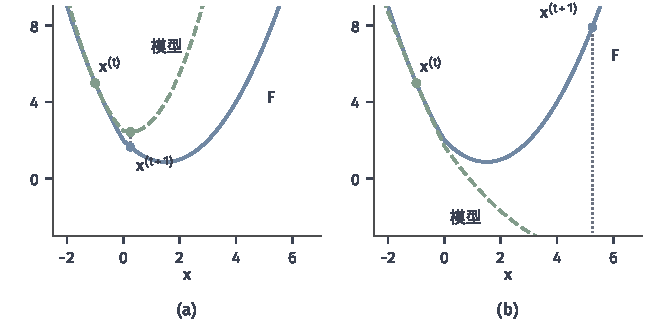
\includegraphics[width=112mm]{figures/05-optimization/03-nonsmooth-optimization/matplotlib/ns-composite-model/figure.pdf}
  \caption{复合目标的局部模型，$F(x)=\tfrac12(x-2)^2+\tfrac12\lvert x\rvert$，$L=1$，当前点$x^{(t)}=-1$。蓝线是$F$，绿色虚线是式~\eqref{eq:ns-composite-model}的模型，蓝点是新点处的真实目标值。(a)$\alpha=0.5$，模型在$F$上方，新点$x^{(t+1)}=0.25$处$F$从$5$降到约$1.66$。(b)$\alpha=2.5$，模型部分低于$F$，新点$x^{(t+1)}=5.25$处$F$升到约$7.9$。}
  \label{fig:ns-composite-model}
\end{BookInlineFigure}

式~\eqref{eq:ns-prox-grad}包含几种已知情形：$r=0$时是梯度下降；$f=0$时是邻近点法；$r=\iota_{\bm{C}}$时是投影梯度法，集合的计算和可行点的最优性将在第~\ref{chap:feasible-iterations}章讨论。

取$r=\lambda\lVert\cdot\rVert_1$（$\lambda>0$），$f$为Lasso的最小二乘项，$\nabla f(\bm{x})=\bm{A}^\top(\bm{A}\bm{x}-\bm{b})$，$L=\lVert\bm{A}\rVert_2^2$。由软阈值式~\eqref{eq:ns-soft-threshold}，邻近步的阈值是步长乘$\lambda$，式~\eqref{eq:ns-prox-grad}成为
\begin{equation}
 \bm{x}^{(t+1)}=S_{\alpha\lambda}\bigl(\bm{x}^{(t)}-\alpha\bm{A}^\top(\bm{A}\bm{x}^{(t)}-\bm{b})\bigr).
 \label{eq:ns-ista}
\end{equation}

这种迭代称为\term{迭代软阈值算法}（iterative shrinkage-thresholding algorithm，ISTA）。“迭代”和“阈值”正好是它的两步：先按最小二乘的方向修正系数，再把小的系数压成零。

\paragraph{计算过程}
用章首的例~\eqref{eq:ns-lasso-example}。

\needspace{6\baselineskip}
\paragraph{变量}
\begin{itemize}
 \item $\bm{A}\in\mathbb{R}^{p\times n}$，$\bm{b}\in\mathbb{R}^p$，$\lambda>0$：数据。例中$p=3$，$n=2$，$\lambda=1$。
 \item $\bm{x}^{(t)}\in\mathbb{R}^n$：当前点。
 \item $\bm{g}^{(t)}$：光滑项在当前点的梯度。
 \item $\alpha$：步长，$\alpha\leq1/L$。
\end{itemize}

\paragraph{初始化}
选$\bm{x}^{(0)}$和$\alpha$。例中$\bm{A}^\top\bm{A}$和$\bm{A}^\top\bm{b}$分别是
\[
 \bm{A}^\top\bm{A}=\begin{pmatrix}2&1\\1&2\end{pmatrix},\qquad\bm{A}^\top\bm{b}=\begin{pmatrix}5\\2\end{pmatrix}.
\]
$\bm{A}^\top\bm{A}$的特征值是$3$和$1$，所以$L=3$。取$\alpha=1/3$，$\bm{x}^{(0)}=(0,0)$，阈值$\alpha\lambda=1/3$。

\needspace{6\baselineskip}
\paragraph{每轮更新}
\begin{enumerate}
 \item 算梯度，$\bm{g}^{(t)}$等于$\bm{A}^\top\bm{A}\bm{x}^{(t)}$减去$\bm{A}^\top\bm{b}$。例中第一轮
 \[
  \bm{g}^{(0)}=(-5,-2).
 \]
 \item 走梯度步$\bm{z}^{(t)}=\bm{x}^{(t)}-\alpha\bm{g}^{(t)}$。例中第一轮
 \[
  \bm{z}^{(0)}=\Bigl(\frac53,\ \frac23\Bigr).
 \]
 \item 逐坐标软阈值，由式~\eqref{eq:ns-ista}得新点。例中第一轮
 \[
  \bm{x}^{(1)}=\Bigl(\frac43,\ \frac13\Bigr),\qquad F(\bm{x}^{(1)})=\frac{11}{3}.
 \]
\end{enumerate}

第二轮的三个量依次是
\[
 \bm{g}^{(1)}=(-2,\,0),\qquad\bm{z}^{(1)}=\Bigl(2,\ \frac13\Bigr),\qquad\bm{x}^{(2)}=\Bigl(\frac53,\ 0\Bigr).
\]

第二分量恰好被压到零。第三轮的三个量依次是
\[
 \bm{g}^{(2)}=\Bigl(-\frac53,\,-\frac13\Bigr),\qquad\bm{z}^{(2)}=\Bigl(\frac{20}{9},\ \frac19\Bigr),\qquad\bm{x}^{(3)}=\Bigl(\frac{17}{9},\ 0\Bigr).
\]

此后第二分量一直为零：$\bm{z}$的第二分量是$(2-x_1)/3$，绝对值小于阈值$1/3$。第一分量满足$x_1^{+}=x_1/3+4/3$，每轮把与$2$的距离缩小三分之一。目标差依次是
\[
 \frac23,\qquad\frac19,\qquad\frac{1}{81},\qquad\frac{1}{729},\ldots
\]

达到预定的迭代次数或后面第~\ref{sec:ns-stopping}小节的停止条件后结束，最终得到$\bm{x}^{(T)}\to(2,0)$，也就是第~\ref{sec:ns-subdifferential}节验证的解。

\paragraph{收敛分析}
分析的核心是一步不等式，把式~\eqref{eq:ns-prox-characterization}与下降引理结合。

\begin{lemma}[邻近梯度的一步不等式]
\label{lem:ns-pg-one-step}
设$f$凸且可微，$r$是适当、下半连续的凸函数，$F=f+r$。给定$\bm{y}$与$\alpha>0$，令
\begin{equation}
 \bm{x}^{+}=\operatorname{prox}_{\alpha r}\bigl(\bm{y}-\alpha\nabla f(\bm{y})\bigr).
 \label{eq:ns-pg-step-y}
\end{equation}
若
\begin{equation}
 f(\bm{x}^{+})\leq f(\bm{y})+\langle\nabla f(\bm{y}),\bm{x}^{+}-\bm{y}\rangle+\frac{1}{2\alpha}\lVert\bm{x}^{+}-\bm{y}\rVert_2^2,
 \label{eq:ns-backtrack-condition}
\end{equation}
则对任意$\bm{z}\in\operatorname{dom}F$，
\begin{equation}
 F(\bm{x}^{+})-F(\bm{z})\leq\frac{1}{2\alpha}\Bigl(\lVert\bm{y}-\bm{z}\rVert_2^2-\lVert\bm{x}^{+}-\bm{z}\rVert_2^2\Bigr).
 \label{eq:ns-pg-one-step}
\end{equation}
\end{lemma}

\begin{proof}
$f$的凸性给出下界
\[
 f(\bm{y})+\langle\nabla f(\bm{y}),\bm{z}-\bm{y}\rangle\leq f(\bm{z}).
\]
把它代入式~\eqref{eq:ns-backtrack-condition}，
\[
 f(\bm{x}^{+})\leq f(\bm{z})+\langle\nabla f(\bm{y}),\bm{x}^{+}-\bm{z}\rangle+\frac{1}{2\alpha}\lVert\bm{x}^{+}-\bm{y}\rVert_2^2.
\]

由式~\eqref{eq:ns-prox-characterization}和式~\eqref{eq:ns-pg-step-y}，下面的$\bm{s}$是$r$在$\bm{x}^{+}$的次梯度：
\[
 \bm{s}=\frac{\bm{y}-\bm{x}^{+}}{\alpha}-\nabla f(\bm{y}).
\]
所以
\[
 r(\bm{x}^{+})\leq r(\bm{z})+\langle\bm{s},\bm{x}^{+}-\bm{z}\rangle.
\]

两式相加，$\nabla f(\bm{y})$的项相消，得到
\[
 F(\bm{x}^{+})\leq F(\bm{z})+\frac{1}{\alpha}\langle\bm{y}-\bm{x}^{+},\bm{x}^{+}-\bm{z}\rangle+\frac{1}{2\alpha}\lVert\bm{x}^{+}-\bm{y}\rVert_2^2.
\]

再用恒等式~\eqref{eq:ns-three-point}，令$\bm{a}=\bm{y}$，$\bm{b}=\bm{x}^{+}$，$\bm{c}=\bm{z}$，最后一项被抵消，就是式~\eqref{eq:ns-pg-one-step}。
\end{proof}

条件~\eqref{eq:ns-backtrack-condition}只在$\bm{y}$和$\bm{x}^{+}$这一对点上要求上界成立，$\alpha\leq1/L$时自动满足。下面的结论就是这个引理对$\bm{y}=\bm{x}^{(t)}$的累加。

\begin{theorem}[邻近梯度法的收敛速率]
\label{thm:ns-pg-rate}
设$f$凸，梯度$L$-Lipschitz连续，$r$是适当、下半连续的凸函数，$F$存在最小点$\bm{x}^\star$，每步精确计算邻近映射，$0<\alpha\leq1/L$。则$F(\bm{x}^{(t)})$单调不增，并且
\begin{equation}
 F(\bm{x}^{(T)})-F^\star\leq\frac{\lVert\bm{x}^{(0)}-\bm{x}^\star\rVert_2^2}{2\alpha T}.
 \label{eq:ns-pg-rate}
\end{equation}
\end{theorem}

\begin{proof}
在式~\eqref{eq:ns-pg-one-step}中取$\bm{y}=\bm{z}=\bm{x}^{(t)}$（$t\geq1$时$\bm{x}^{(t)}\in\operatorname{dom}F$），右端为负，所以$F$单调不增。

取$\bm{y}=\bm{x}^{(t)}$，$\bm{z}=\bm{x}^\star$，对$t=0,\ldots,T-1$相加，距离项相消，得到
\[
 \sum_{t=0}^{T-1}\bigl(F(\bm{x}^{(t+1)})-F^\star\bigr)\leq\frac{\lVert\bm{x}^{(0)}-\bm{x}^\star\rVert_2^2}{2\alpha}.
\]

由单调性，左端每一项都不小于$F(\bm{x}^{(T)})-F^\star$，所以左端不小于$T(F(\bm{x}^{(T)})-F^\star)$，即得式~\eqref{eq:ns-pg-rate}。
\end{proof}

速率$O(1/T)$与第~\ref{chap:first-order-methods}章的梯度下降相同，比次梯度法的$O(1/\sqrt{T})$快得多，代价是$r$的邻近映射必须算得出。这里$\bm{x}^{(0)}$若不在$\operatorname{dom}r$，第一步的邻近映射会把点带入定义域，定理依然成立。

例中$R^2=\lVert\bm{x}^{(0)}-\bm{x}^\star\rVert_2^2=4$，$\alpha=1/3$，界为$6/T$，$T=3$时为$2$。实际目标差$1/81$小得多，因为一旦$x_2$落到零，迭代实际上在一维的强凸二次函数上运行，收敛是线性的。这也是Lasso上常见的现象：大多数轮次之后，支撑集（非零分量的位置）不再变化，算法此后近似一个定义在支撑集上的光滑问题。

\subsection{加速邻近梯度法（FISTA）}
\label{sec:ns-fista}

第~\ref{chap:first-order-methods}章的Nesterov方法把光滑凸目标的速率从$1/T$提高到$1/T^2$，代价只是多存一个向量。本小节要回答：这种外推能否直接搬到复合目标上？

\paragraph{主要思想}
把Nesterov方法里的梯度步换成邻近梯度步，外推系数原样保留。这就是\term{加速邻近梯度法}（fast iterative shrinkage-thresholding algorithm，FISTA）\scite{beck2009fista}：
\begin{equation}
 \begin{aligned}
 \bm{x}^{(t+1)}&=\operatorname{prox}_{\alpha r}\bigl(\bm{y}^{(t)}-\alpha\nabla f(\bm{y}^{(t)})\bigr),\\
 \bm{y}^{(t+1)}&=\bm{x}^{(t+1)}+\frac{\theta^{(t)}-1}{\theta^{(t+1)}}\bigl(\bm{x}^{(t+1)}-\bm{x}^{(t)}\bigr).
 \end{aligned}
 \label{eq:ns-fista}
\end{equation}

其中$\bm{y}^{(0)}=\bm{x}^{(0)}$，$\theta^{(0)}=1$，外推参数按第~\ref{chap:first-order-methods}章的递推更新：
\begin{equation}
 \theta^{(t+1)}=\frac{1+\sqrt{1+4(\theta^{(t)})^2}}{2}.
 \label{eq:ns-fista-theta}
\end{equation}
图~\ref{fig:ns-fista-structure}是一步的结构：先沿上一步位移外推到$\bm{y}^{(t)}$，在外推点读梯度，再做邻近步。梯度必须取在$\bm{y}^{(t)}$，这是Nesterov方法的特点，与重球法不同。

\begin{BookInlineFigure}
  \centering
  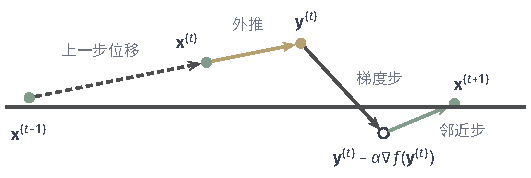
\includegraphics[width=89.9mm]{figures/05-optimization/03-nonsmooth-optimization/tikz/ns-fista-structure/figure.pdf}
  \caption{FISTA的一步。黄色外推从$\bm{x}^{(t)}$沿上一步位移（虚线）走到$\bm{y}^{(t)}$，深灰箭头是在$\bm{y}^{(t)}$处的梯度步，绿色箭头是邻近步，可能把点压回坐标面（深灰横线）。空心圆是梯度步的终点。}
  \label{fig:ns-fista-structure}
\end{BookInlineFigure}

\paragraph{计算过程}
仍用例~\eqref{eq:ns-lasso-example}，$\alpha=1/3$，阈值$1/3$。

\needspace{6\baselineskip}
\paragraph{变量}
\begin{itemize}
 \item $\bm{x}^{(t)}$：邻近步的输出，是算法报告的点。
 \item $\bm{y}^{(t)}$：外推点，形状与$\bm{x}$相同，读梯度在这里。
 \item $\theta^{(t)}$：外推参数。
\end{itemize}

\paragraph{初始化}
$\bm{x}^{(0)}=\bm{y}^{(0)}=\bm{0}$，$\theta^{(0)}=1$。

\needspace{6\baselineskip}
\paragraph{每轮更新}
\begin{enumerate}
 \item 在$\bm{y}^{(t)}$读梯度并做邻近梯度步，由式~\eqref{eq:ns-fista}得$\bm{x}^{(t+1)}$。例中第一轮$\bm{y}^{(0)}=\bm{0}$，结果与ISTA相同：
 \[
  \bm{x}^{(1)}=\Bigl(\frac43,\ \frac13\Bigr).
 \]
 \item 更新$\theta^{(t+1)}$。例中第一轮
 \[
  \theta^{(1)}=\frac{1+\sqrt5}{2}\approx1.618.
 \]
 \item 计算外推点。例中第一轮系数$(\theta^{(0)}-1)/\theta^{(1)}=0$，所以$\bm{y}^{(1)}=\bm{x}^{(1)}$。
\end{enumerate}

第二轮仍无外推差别，同样得到$\bm{x}^{(2)}=(5/3,0)$。这时开始用上外推，
\[
 \theta^{(2)}\approx2.194,\qquad\frac{\theta^{(1)}-1}{\theta^{(2)}}\approx0.282.
\]

外推点是
\[
 \bm{y}^{(2)}=\Bigl(\frac53,0\Bigr)+0.282\Bigl(\frac13,-\frac13\Bigr)\approx(1.761,\,-0.094).
\]

第三轮的梯度、梯度步和新点依次是
\[
 \begin{gathered}
 \nabla f(\bm{y}^{(2)})\approx(-1.573,\,-0.427),\qquad
 \bm{z}\approx(2.285,\,0.048),\\
 \bm{x}^{(3)}\approx(1.952,\,0).
 \end{gathered}
\]

与ISTA的$17/9\approx1.889$相比更接近$2$，目标差约$0.0024$，ISTA是$0.0123$。外推的好处在第三轮就看得到了。

继续迭代，第一分量在第$4$轮越过$2$到达约$2.025$，然后缓慢摆回，目标差从第$7$轮的约$1.2\times10^{-6}$升到第$8$轮的约$4.4\times10^{-6}$。这个小问题上$\kappa=3$，ISTA已经很快，FISTA并不占优，但它显示了FISTA的目标值不是逐轮下降的。图~\ref{fig:ns-ista-path}对比了两条路径。

\begin{BookInlineFigure}
  \centering
  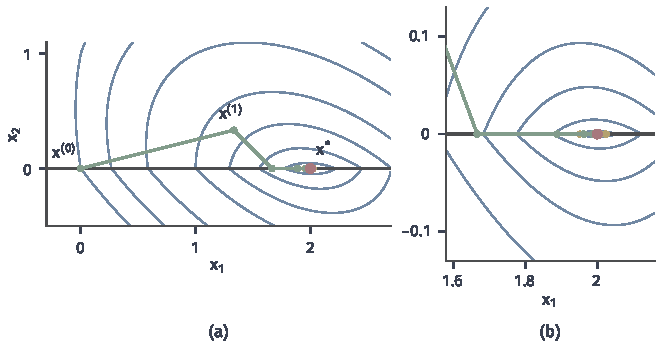
\includegraphics[width=112mm]{figures/05-optimization/03-nonsmooth-optimization/matplotlib/ns-ista-path/figure.pdf}
  \caption{贯穿例~\eqref{eq:ns-lasso-example}上的ISTA（绿）与FISTA（黄），蓝线是$F$的等高线，深灰横线是尖点所在的$x_2=0$。(a)全貌，迭代很快落到$x_2=0$上，等高线在这条线上带角。(b)$\bm{x}^\star=(2,0)$附近放大，FISTA越过红点后又摆回。}
  \label{fig:ns-ista-path}
\end{BookInlineFigure}

\paragraph{收敛分析}
结论的形式与第~\ref{chap:first-order-methods}章相同，证明把那里的一步不等式换成引理~\ref{lem:ns-pg-one-step}。我们把比较点写成任意的$\bm{z}$，后面分析光滑化时要用这个写法。

\begin{theorem}[FISTA的收敛速率]
\label{thm:ns-fista-rate}
设$f$凸，梯度$L$-Lipschitz连续，$r$是适当、下半连续的凸函数，每步精确计算邻近映射，$\alpha=1/L$，$\theta^{(t)}$按式~\eqref{eq:ns-fista-theta}递推。则对任意$\bm{z}\in\operatorname{dom}F$和$T\geq1$，
\begin{equation}
 F(\bm{x}^{(T)})-F(\bm{z})\leq\frac{2L\lVert\bm{x}^{(0)}-\bm{z}\rVert_2^2}{(T+1)^2}.
 \label{eq:ns-fista-rate}
\end{equation}
特别地，若$F$存在最小点$\bm{x}^\star$，取$\bm{z}=\bm{x}^\star$就得到目标差界。
\end{theorem}

\begin{proof}
记$\theta=\theta^{(t)}$，$\Delta_t$为目标差$F(\bm{x}^{(t)})-F(\bm{z})$。在引理~\ref{lem:ns-pg-one-step}中取$\bm{y}=\bm{y}^{(t)}$，$\bm{x}^{+}=\bm{x}^{(t+1)}$，比较点取
\[
 \bm{v}=\Bigl(1-\frac1\theta\Bigr)\bm{x}^{(t)}+\frac1\theta\bm{z}.
\]

由$F$的凸性，
\[
 F(\bm{v})-F(\bm{z})\leq\Bigl(1-\frac1\theta\Bigr)\Delta_t.
\]

代入式~\eqref{eq:ns-pg-one-step}，并记$\alpha=1/L$，得
\[
 \Delta_{t+1}-\Bigl(1-\frac1\theta\Bigr)\Delta_t\leq\frac L2\Bigl(\lVert\bm{y}^{(t)}-\bm{v}\rVert_2^2-\lVert\bm{x}^{(t+1)}-\bm{v}\rVert_2^2\Bigr).
\]

两边乘$\theta^2$，把$\theta$乘进范数。定义
\[
 \bm{u}^{(t+1)}=\theta^{(t)}\bm{x}^{(t+1)}-(\theta^{(t)}-1)\bm{x}^{(t)}-\bm{z},
\]
则$\theta\bm{x}^{(t+1)}-\theta\bm{v}=\bm{u}^{(t+1)}$。

再看另一项。令$\bm{u}^{(0)}=\bm{x}^{(0)}-\bm{z}$。由外推式~\eqref{eq:ns-fista}，$t\geq1$时有
\[
 \theta^{(t)}\bm{y}^{(t)}=\theta^{(t)}\bm{x}^{(t)}+(\theta^{(t-1)}-1)(\bm{x}^{(t)}-\bm{x}^{(t-1)}),
\]
于是
\[
 \theta\bm{y}^{(t)}-\theta\bm{v}=\bm{u}^{(t)}.
\]
$t=0$时$\theta^{(0)}=1$，$\bm{y}^{(0)}=\bm{x}^{(0)}$，同一等式也成立。

由递推，$\theta^2-\theta=(\theta^{(t-1)})^2$（$t\geq1$），而$t=0$时$\theta^2-\theta=0$。代入不等式，得到势函数的单调性：
\[
 (\theta^{(t)})^2\Delta_{t+1}+\frac L2\lVert\bm{u}^{(t+1)}\rVert_2^2\leq(\theta^{(t-1)})^2\Delta_t+\frac L2\lVert\bm{u}^{(t)}\rVert_2^2.
\]

把它从$t=T-1$一直用到$t=0$，最后一步$\theta^2-\theta=0$使$\Delta_0$的项消失，于是
\[
 (\theta^{(T-1)})^2\Delta_T\leq\frac L2\lVert\bm{x}^{(0)}-\bm{z}\rVert_2^2.
\]

由$\theta^{(t)}\geq(t+2)/2$得$(\theta^{(T-1)})^2\geq(T+1)^2/4$，代入即得结论。
\end{proof}

证明里没有用到$\Delta_t$的符号，这也是比较点可以取任意$\bm{z}$的原因。下面三点是使用时要注意的。第一，界里的$F(\bm{x}^{(T)})$不要求逐轮下降，例中第$8$轮的回升就是证据；若需要单调，可以在每轮比较后保留较好的点，但这样改过的算法需要另外分析。第二，$\alpha=1/L$可以换成回溯，但证明要求步长不增。第三，这个证明用到$F$的凸性（比较点$\bm{v}$的那一步），不能直接用于非凸的$f$。

图~\ref{fig:ns-ista-fista-rates}用一个条件更差的问题（$100\times200$的相关设计矩阵）比较两种方法。ISTA在这种问题上明显受制于条件数，FISTA在更少的迭代内到达更低的目标差，代价是目标值的振荡。

\begin{BookInlineFigure}
  \centering
  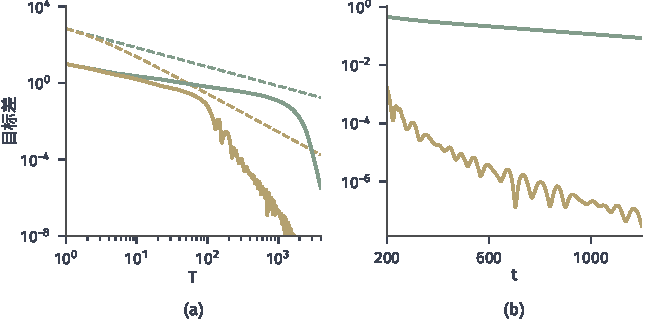
\includegraphics[width=112mm]{figures/05-optimization/03-nonsmooth-optimization/matplotlib/ns-ista-fista-rates/figure.pdf}
  \caption{相关设计的Lasso上的ISTA（绿）与FISTA（黄）。$\bm{A}\in\mathbb{R}^{100\times200}$的列间相关系数$\rho=0.9$，$\lambda$取为$0.005\lVert\bm{A}^\top\bm{b}\rVert_\infty$，$\alpha=1/L$。(a)目标差（双对数），同色虚线是定理~\ref{thm:ns-pg-rate}与定理~\ref{thm:ns-fista-rate}的上界。(b)第$200$到第$1200$轮的放大（半对数），FISTA的目标差呈周期性振荡，ISTA单调下降。最优值由高精度运行得到。}
  \label{fig:ns-ista-fista-rates}
\end{BookInlineFigure}

\subsection{停止条件与计算成本}
\label{sec:ns-stopping}

算法要在不知道$F^\star$的情况下决定何时停止。无约束光滑问题有$\lVert\nabla f\rVert_2$，复合目标在尖点上没有梯度，需要一个可计算的残差。本小节回答：这个残差是什么，它小意味着什么，以及比较算法时要算哪些账。

\paragraph{邻近梯度映射}
把一步更新的位移除以步长，定义\term{邻近梯度映射}（proximal gradient mapping）
\begin{equation}
 \bm{G}_\alpha(\bm{x})=\frac{1}{\alpha}\Bigl(\bm{x}-\operatorname{prox}_{\alpha r}\bigl(\bm{x}-\alpha\nabla f(\bm{x})\bigr)\Bigr).
 \label{eq:ns-gradient-mapping}
\end{equation}

$r=0$时它就是$\nabla f(\bm{x})$，所以它是梯度在复合目标上的替身。更新可以写成$\bm{x}^{+}=\bm{x}-\alpha\bm{G}_\alpha(\bm{x})$，这样它和梯度步在形式上完全一样。第~\ref{chap:optimization}章提到的非光滑问题的最优性残差，就是这个量。

满足$\bm{0}\in\nabla f(\bm{x})+\partial r(\bm{x})$的点称为\term{复合驻点}（composite stationary point）。这个定义不要求$f$凸。

\begin{theorem}[映射残差的含义]
\label{thm:ns-residual}
设$f$梯度$L$-Lipschitz连续，$r$是适当、下半连续的凸函数，$\alpha>0$，$\bm{x}^{+}=\bm{x}-\alpha\bm{G}_\alpha(\bm{x})$。
\begin{enumerate}
 \item $\bm{G}_\alpha(\bm{x})=\bm{0}$当且仅当$\bm{x}$是复合驻点。
 \item 若$f$凸且$\bm{G}_\alpha(\bm{x})=\bm{0}$，则$\bm{x}$是$F$的全局最小点。
 \item 若$\alpha L\leq1$，则$\bm{G}_\alpha(\bm{x})+\nabla f(\bm{x}^{+})-\nabla f(\bm{x})\in\nabla f(\bm{x}^{+})+\partial r(\bm{x}^{+})$，且范数不超过$2\lVert\bm{G}_\alpha(\bm{x})\rVert_2$。$f$凸且最小点$\bm{x}^\star$存在时，
 \begin{equation}
  F(\bm{x}^{+})-F^\star\leq2\lVert\bm{G}_\alpha(\bm{x})\rVert_2\,\lVert\bm{x}^{+}-\bm{x}^\star\rVert_2.
  \label{eq:ns-residual-gap}
 \end{equation}
 \item 不要求$f$凸，$\alpha=1/L$，$F$有下界$F_{\inf}$时，邻近梯度法满足
 \begin{equation}
  \min_{0\leq t<T}\lVert\bm{G}_\alpha(\bm{x}^{(t)})\rVert_2^2\leq\frac{2L\bigl(F(\bm{x}^{(0)})-F_{\inf}\bigr)}{T}.
  \label{eq:ns-nonconvex-residual}
 \end{equation}
\end{enumerate}
\end{theorem}

\begin{proof}
由式~\eqref{eq:ns-prox-characterization}，$\bm{x}^{+}$由下式刻画：
\[
 \bm{G}_\alpha(\bm{x})-\nabla f(\bm{x})\in\partial r(\bm{x}^{+}).
\]

第一条：$\bm{G}_\alpha(\bm{x})=\bm{0}$时$\bm{x}^{+}=\bm{x}$，上式就是$-\nabla f(\bm{x})\in\partial r(\bm{x})$。反过来，若$-\nabla f(\bm{x})\in\partial r(\bm{x})$，则由式~\eqref{eq:ns-prox-characterization}，$\bm{x}$本身就是$\bm{x}-\alpha\nabla f(\bm{x})$的邻近点，所以$\bm{x}^{+}=\bm{x}$。

第二条：$f$凸时$\partial F=\nabla f+\partial r$，用定理~\ref{thm:ns-fermat}。

第三条：在上式两边加$\nabla f(\bm{x}^{+})$就得到前半部分。范数方面，
\[
 \lVert\nabla f(\bm{x}^{+})-\nabla f(\bm{x})\rVert_2\leq L\lVert\bm{x}^{+}-\bm{x}\rVert_2=L\alpha\lVert\bm{G}_\alpha(\bm{x})\rVert_2\leq\lVert\bm{G}_\alpha(\bm{x})\rVert_2.
\]
$f$凸时这个向量是$F$在$\bm{x}^{+}$的次梯度，用支撑不等式和Cauchy不等式，得到式~\eqref{eq:ns-residual-gap}。

第四条：由刻画式和次梯度不等式，
\[
 r(\bm{x})\geq r(\bm{x}^{+})+\langle\bm{G}_\alpha(\bm{x})-\nabla f(\bm{x}),\bm{x}-\bm{x}^{+}\rangle.
\]

代入$\bm{x}-\bm{x}^{+}=\alpha\bm{G}_\alpha(\bm{x})$。再用下降引理
\[
 f(\bm{x}^{+})\leq f(\bm{x})+\langle\nabla f(\bm{x}),\bm{x}^{+}-\bm{x}\rangle+\frac L2\lVert\bm{x}^{+}-\bm{x}\rVert_2^2.
\]
两式相加，当$\alpha=1/L$时得到
\[
 F(\bm{x}^{+})\leq F(\bm{x})-\frac{1}{2L}\lVert\bm{G}_\alpha(\bm{x})\rVert_2^2.
\]
对$t$求和，就是式~\eqref{eq:ns-nonconvex-residual}。
\end{proof}

第三条给出了可计算的证书：$\bm{x}^{+}$处的一个具体的次梯度，其范数不超过$2\lVert\bm{G}\rVert$。第四条说明非凸时没有目标差界，只能保证残差变小，这与光滑非凸问题的情况相同。

非凸时残差为零不代表最优。取$f(x)=-x^2/2$，$r=\iota_{[-1,1]}$，$L=1$，$\alpha=1$，则
\[
 G_1(x)=x-\Pi_{[-1,1]}(2x).
\]
$x=0$处$G_1=0$，但$0$是这个问题的最大点，真正的最优解在$\pm1$。

用贯穿例核对第三条。ISTA在$\bm{x}^{(3)}=(17/9,0)$处的下一步是$\bm{x}^{(4)}=(53/27,0)$，所以
\[
 \bm{G}_{1/3}(\bm{x}^{(3)})=3\Bigl(\frac{17}{9}-\frac{53}{27},\ 0\Bigr)=\Bigl(-\frac29,\ 0\Bigr).
\]

式~\eqref{eq:ns-residual-gap}的右端是$2\cdot\tfrac29\cdot\tfrac{1}{27}\approx0.0165$，实际$F(\bm{x}^{(4)})-F^\star\approx0.00137$，上界成立。

\paragraph{停止条件}
实际常用的停止条件是残差相对于初始残差足够小：
\begin{equation}
 \lVert\bm{G}_\alpha(\bm{x}^{(t)})\rVert_2\leq\varepsilon\max\bigl\{1,\lVert\bm{G}_\alpha(\bm{x}^{(0)})\rVert_2\bigr\}.
 \label{eq:ns-stopping}
\end{equation}

FISTA的邻近梯度步是在$\bm{y}^{(t)}$处算的，$\bm{G}_\alpha(\bm{y}^{(t)})$可以免费得到；若要在$\bm{x}^{(t)}$处的残差，需要多算一次梯度和邻近映射。图~\ref{fig:ns-residual-restart}(a)显示，FISTA的残差并不单调，单轮的残差读数可能偶然偏小，稳妥的做法是连续多轮满足条件才停止。

\paragraph{回溯}
$L$未知或局部$L$远小于全局$L$时，用回溯确定$\alpha$。关键是在实际读梯度的点上检验二次上界，对FISTA这个点是$\bm{y}^{(t)}$，不是$\bm{x}^{(t)}$。

回溯的做法是：取当前$\alpha$，由式~\eqref{eq:ns-pg-step-y}计算$\bm{x}^{+}$，检验条件~\eqref{eq:ns-backtrack-condition}。不满足就令$\alpha\leftarrow\rho\alpha$（$\rho\in(0,1)$）重算邻近步。引理~\ref{lem:ns-pg-one-step}只要求这一对点上的上界，所以条件一满足，一步不等式就成立。FISTA的定理~\ref{thm:ns-fista-rate}还需要步长不增，步长增大后势函数不再相消，这时需要专门设计的$\theta$递推。

\paragraph{不精确的邻近步}
$r$的邻近映射没有闭式解时，子问题要迭代求解。设第$t$步邻近子问题的目标值误差不超过$\epsilon^{(t)}$。已有的结论要求：ISTA的$O(1/T)$需要$\sum_t\sqrt{\epsilon^{(t)}}<\infty$，FISTA的$O(1/T^2)$需要$\sum_tt\sqrt{\epsilon^{(t)}}<\infty$。

FISTA的要求更严：外推把误差放大了，误差必须更快地衰减。这个结论的证明需要把误差项带进势函数分析，篇幅较长。它的实际含义是，加速方法的子问题要解得更准，节省的迭代次数要扣掉更贵的子问题。

\paragraph{重启}
FISTA的外推系数$\beta^{(t)}$趋于$1$，在强凸的方向上动量过大，表现为目标值的振荡。重启是把$\theta$重置为$1$、令$\bm{y}=\bm{x}$，相当于扔掉累积的动量。常用的函数值重启规则是：一旦$F(\bm{x}^{(t+1)})>F(\bm{x}^{(t)})$就重启。

图~\ref{fig:ns-residual-restart}(b)显示，同一问题上重启使收敛快了很多。这个规则的保证要单独核对：定理~\ref{thm:ns-fista-rate}是从一次连续运行中得到的，重启之后势函数归零，$1/T^2$的总界不能直接沿用。每一段的界仍然成立，段长由规则决定；若目标在解附近有二次增长，可以证明周期重启得到线性收敛。如果每步都重启，FISTA退化成ISTA。

\begin{BookInlineFigure}
  \centering
  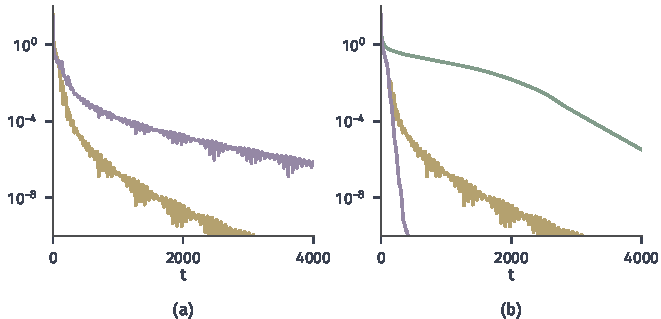
\includegraphics[width=112mm]{figures/05-optimization/03-nonsmooth-optimization/matplotlib/ns-residual-restart/figure.pdf}
  \caption{FISTA的残差与重启，问题与图~\ref{fig:ns-ista-fista-rates}相同（半对数坐标）。(a)黄线是目标差，紫线是$\bm{x}^{(t)}$处的映射残差范数，两者都不单调。(b)绿线是ISTA，黄线是FISTA，紫线是带函数值重启的FISTA。}
  \label{fig:ns-residual-restart}
\end{BookInlineFigure}

\paragraph{成本对比}
比较ISTA和FISTA时，把一次迭代的成本拆开。

\begin{BookInlineTable}
  \centering
  \small
  \begin{tabular}{@{}lll@{}}
    \toprule
     & ISTA & FISTA\\
    \midrule
    每步梯度 & $1$次，在$\bm{x}^{(t)}$ & $1$次，在$\bm{y}^{(t)}$\\
    每步邻近映射 & $1$次 & $1$次\\
    额外存储 & 无 & $\bm{x}^{(t-1)}$与$\bm{y}^{(t)}$\\
    回溯 & 每次试探增加$1$次邻近、$1$次$f$ & 同左，试探点是$\bm{y}^{(t)}$\\
    目标值单调 & 是 & 否\\
    目标差界 & $O(1/T)$ & $O(1/T^2)$\\
    非凸$f$ & 残差界式~\eqref{eq:ns-nonconvex-residual} & 无此保证\\
    \bottomrule
  \end{tabular}
  \caption{ISTA与FISTA的成本和保证。计算函数值用于重启或停止时，FISTA每轮还要加上一次$F$的计算。}
  \label{tab:ns-ista-fista}
\end{BookInlineTable}

对Lasso，一次梯度$\bm{A}^\top(\bm{A}\bm{x}-\bm{b})$是两次矩阵向量乘，一次软阈值只要$O(n)$。主要成本在矩阵向量乘，所以“迭代次数”可以当作比较的单位。当邻近映射本身要迭代时，这个单位就不合适了，比较必须按总的基本运算数，见表~\ref{tab:ns-ista-fista}。
